\documentclass[main.tex]{subfiles}
\begin{document}
	
	The method presented in this \paper{} performs static code analysis on Haskell modules to determine which extensions are needed in the module, and which ones are not. For this, the algorithm needs an abstract representation of the source code. This representation is called the \emph{abstract syntax tree}, shortly referred to as \emph{AST}. The syntax tree can be constructed by an external tool, such as \cite{haskell-src-exts} or by the compiler itself. The algorithm presented here uses a syntax tree produced by a combination of these two techniques. It uses the unique representation of Haskell-Tools, which is a transformed version of the GHC syntax tree. In Diagram~\ref{fig:haskell-tools-architecture}\footnote{The diagram is taken from the Haskell-Tools \href{https://github.com/haskell-tools/haskell-tools/blob/master/documentation/haskell_tools_architecture.png}{documentation}. April 29, 2018 } we can see the outline of Haskell-Tools' architecture. In this chapter, we will discuss the various properties of the Haskell-Tools AST and present a general overview of its construction. The work described in the following sections is not part of this \paper{}. 
	
	\begin{figure}[H]
		\renewcommand{\figurename}{Diagram}
		\hspace{-1cm}
		\centering
		\caption{Architecture of Haskell-Tools}
		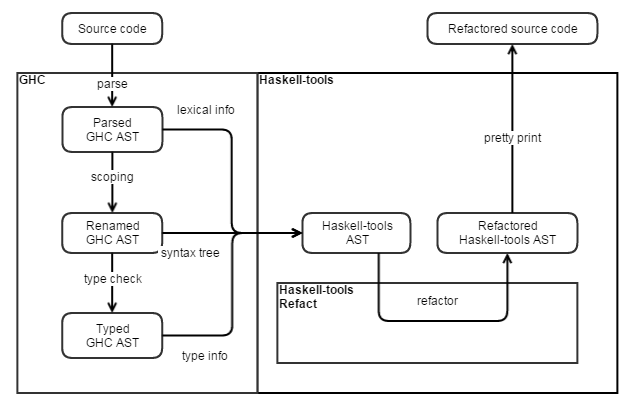
\includegraphics[scale=0.5]{haskell_tools_architecture}
		\label{fig:haskell-tools-architecture}
	\end{figure}
	
	\newpage
	
	\section{Properties of the abstract syntax tree}
	
	Despite its name, the syntax tree can contain much more information about the source code than only its syntactic structure. The individual extension checkers use two special properties of the syntax tree provided by Haskell-Tools: the semantic information carried by its nodes and also its concrete representation of the source code's syntax.
	
	\subsection{Semantic information}
	
	% semantic X vs semantical X:
	% Ask the question the: does X have meaning? If YES -> semantical, if NO -> semantical
	% semantic object, semantical ambiguity
	
	In most cases, eliminating a certain extension requires more than a syntactic analysis of the source code. From the perspective of the algorithm, the most relevant piece is the semantic information stored in the AST's nodes. There are two kinds of semantic information in the syntax tree that are particularly important: type information and unique names. As discussed in Section~\ref{ghc-exts}, some extensions can enrich the type system of GHC by new features. The type information present in certain nodes of the AST are used to determine the necessity of these extensions.
	
	In the syntax tree, not all nodes have type information associated with them. The reason for this is that the type checker discards intermediate result types after calculating them. As a result, the type information of subexpressions are lost after the type checking phase ends. As a consequence, GHC does not store type information for subexpressions, only for named program elements. In particular, only overloaded literals have directly accessible type information. Luckily, we can obtain the types of other nodes as well by using their unique names. GHC provides certain lookup functions which can recover the type of a given node based on its unique name. Haskell-Tools stores these unique names in the corresponding AST nodes. Unfortunately, using this approach, we can only access the type information of syntax tree nodes with qualified names. For instance, in the example below we can only determine the types of the function \ilcode{f}, the operator \ilcode{(:)} and the variables \ilcode{x} and \ilcode{xs}. We have no information about the subexpressions such as \ilcode{f x}.
	
	\begin{oneLineHaskell}
		map f (x:xs) = f x : map f xs
	\end{oneLineHaskell}
	
	Due to partially available type information, the individual extension checkers can only approximate the necessities of their corresponding language extensions. The algorithm presented in Section~\ref{algorithm} overcomes this issue by introducing so-called \emph{extension formulas} and \emph{certainty levels}. Using these two new constructs, despite the incomplete type information, we can eliminate most unused extensions from Haskell modules, and highlight the language elements requiring the remaining extensions.
	
	\subsection{Concrete syntax}
	
	In addition to the semantically important abstract syntax, the AST of Haskell-Tools also represents the concrete syntax of the source code. One of the main advantages of this approach, is that all the syntactic sugar present in the source code is also present in the AST. This makes the requirement checking of syntactic extensions particularly simple. Since syntactic extensions mostly only introduce some sort of syntactic sugar to the language, we only need to check the presence of the nodes corresponding to the syntactic sugar in the AST.
	
	\section{Constructing the syntax tree}
	
	The abstract syntax tree of Haskell-Tools is constructed from the AST provided by GHC. The transformation process has many different steps from which a few will be briefly outlined in this section.
	
	\subsection{Transforming the GHC representation}
	
	Haskell-Tools aims at optimizing the AST for source code transformation. One of the key steps to achieve this, is collecting all refactoring related information present in the different versions of GHC syntax trees scattered throughout the various stages of compilation. This process is required because in different stages of the compilation GHC stores different kinds of information about the AST. In some cases, between two stages certain information is lost. For example, after the renaming phase, the Template Haskell program elements are no longer present, because they are evaluated.
	
	At a certain point, the semantic information also has to be collected. This phase takes place right after all syntactic parts of the Haskell-Tools AST are constructed. For this transformation Haskell-Tools uses the type checked syntax tree of GHC. It extracts all required information from the GHC representation, and annotates its own AST with it. After the transformation, all nodes in the Haskell-Tools syntax tree will have their corresponding semantic information associated with them. It is also worth mentioning, that not all nodes have semantic information, and different types of nodes may have different types of semantic information. For instance, an operator has its fixity and its qualified name, but a literal has only its type available as semantic information.
	
	
	\subsection{Source related information}
	
	Besides storing the concrete syntactical representation of the source code, Haskell-Tools also keeps track of every bit of source related information present in the program. As a result, the original source code can be obtained from the syntax tree itself. This process is called \emph{pretty printing}. This is a really useful feature, because after performing a refactoring, we can easily generate the source code by pretty printing the syntax tree.
	
	To achieve this kind of behavior, the syntax tree has to go through several stages of transformations where the exact source ranges are calculated for the language elements, and then these ranges are replaced by the corresponding parts of the source code.
	
	
	
\end{document}